\documentclass[14pt]{extbook}
\usepackage{multicol, enumerate, enumitem, hyperref, color, soul, setspace, parskip, fancyhdr} %General Packages
\usepackage{amssymb, amsthm, amsmath, latexsym, units, mathtools} %Math Packages
\everymath{\displaystyle} %All math in Display Style
% Packages with additional options
\usepackage[headsep=0.5cm,headheight=12pt, left=1 in,right= 1 in,top= 1 in,bottom= 1 in]{geometry}
\usepackage[usenames,dvipsnames]{xcolor}
\usepackage{dashrule}  % Package to use the command below to create lines between items
\newcommand{\litem}[1]{\item#1\hspace*{-1cm}\rule{\textwidth}{0.4pt}}
\pagestyle{fancy}
\lhead{Progress Quiz 6}
\chead{}
\rhead{Version C}
\lfoot{9689-6866}
\cfoot{}
\rfoot{Spring 2021}
\begin{document}

\begin{enumerate}
\litem{
Determine the horizontal and/or oblique asymptotes in the rational function below.\[ f(x) = \frac{6x^{3} -13 x^{2} -13 x + 30}{3x^{2} +10 x -25} \]\begin{enumerate}[label=\Alph*.]
\item \( \text{Horizontal Asymptote of } y = 2.0 \text{ and Oblique Asymptote of } y = 2x -11 \)
\item \( \text{Horizontal Asymptote of } y = 2.0  \)
\item \( \text{Oblique Asymptote of } y = 2x -11. \)
\item \( \text{Horizontal Asymptote at } y = -5.0 \)
\item \( \text{Horizontal Asymptote of } y = -5.0 \text{ and Oblique Asymptote of } y = 2x -11 \)

\end{enumerate} }
\litem{
Which of the following functions \textit{could} be the graph below?
\begin{center}
    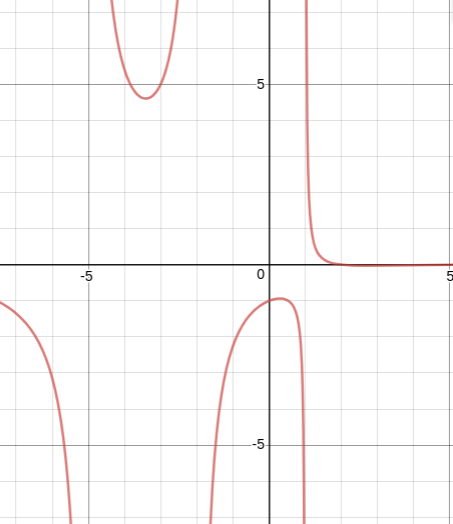
\includegraphics[width=0.5\textwidth]{../Figures/identifyGraphOfRationalFunctionC.png}
\end{center}
\begin{enumerate}[label=\Alph*.]
\item \( f(x)=\frac{x^{3} -7 x^{2} + 36}{x^{3} +2 x^{2} -36 x -72} \)
\item \( f(x)=\frac{x^{3} +2 x^{2} -15 x -36}{x^{3} -2 x^{2} -36 x + 72} \)
\item \( f(x)=\frac{x^{3} -7 x^{2} + 36}{x^{3} +2 x^{2} -36 x -72} \)
\item \( f(x)=\frac{x^{3} +7 x^{2} -36}{x^{3} -2 x^{2} -36 x + 72} \)
\item \( \text{None of the above are possible equations for the graph.} \)

\end{enumerate} }
\litem{
Determine the horizontal and/or oblique asymptotes in the rational function below.\[ f(x) = \frac{2x^{2} +x -6}{12x^{3} -56 x^{2} +17 x + 60} \]\begin{enumerate}[label=\Alph*.]
\item \( \text{Horizontal Asymptote at } y = -2.000 \)
\item \( \text{Horizontal Asymptote of } y = 0 \)
\item \( \text{Horizontal Asymptote of } y = 0.167 \text{ and Oblique Asymptote of } y = 6x -31 \)
\item \( \text{Horizontal Asymptote of } y = 0.167  \)
\item \( \text{Oblique Asymptote of } y = 6x -31. \)

\end{enumerate} }
\litem{
Determine the vertical asymptotes and holes in the rational function below.\[ f(x) = \frac{6x^{3} +29 x^{2} -5 x -100}{8x^{2} +14 x -15} \]\begin{enumerate}[label=\Alph*.]
\item \( \text{Vertical Asymptotes of } x = 0.75 \text{ and } x = -2.5 \text{ with no holes.} \)
\item \( \text{Vertical Asymptotes of } x = 0.75 \text{ and } x = 1.667 \text{ with a hole at } x = -2.5 \)
\item \( \text{Vertical Asymptote of } x = 0.75 \text{ and hole at } x = -2.5 \)
\item \( \text{Holes at } x = 0.75 \text{ and } x = -2.5 \text{ with no vertical asymptotes.} \)
\item \( \text{Vertical Asymptote of } x = 0.75 \text{ and hole at } x = -2.5 \)

\end{enumerate} }
\litem{
Which of the following functions \textit{could} be the graph below?
\begin{center}
    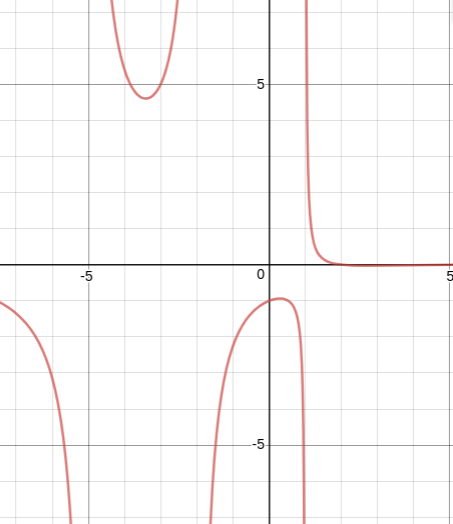
\includegraphics[width=0.5\textwidth]{../Figures/identifyGraphOfRationalFunctionCopyC.png}
\end{center}
\begin{enumerate}[label=\Alph*.]
\item \( f(x)=\frac{x^{3} -4 x^{2} -47 x + 210}{x^{3} +4 x^{2} -31 x -70} \)
\item \( f(x)=\frac{x^{3} -2 x^{2} -36 x + 72}{x^{3} +4 x^{2} -31 x -70} \)
\item \( f(x)=\frac{x^{3} +4 x^{2} -47 x -210}{x^{3} -4 x^{2} -31 x + 70} \)
\item \( f(x)=\frac{x^{3} +4 x^{2} -47 x -210}{x^{3} -4 x^{2} -31 x + 70} \)
\item \( \text{None of the above are possible equations for the graph.} \)

\end{enumerate} }
\litem{
Determine the vertical asymptotes and holes in the rational function below.\[ f(x) = \frac{8x^{3} -30 x^{2} +9 x + 27}{6x^{2} -x -12} \]\begin{enumerate}[label=\Alph*.]
\item \( \text{Vertical Asymptote of } x = -1.333 \text{ and hole at } x = 1.5 \)
\item \( \text{Vertical Asymptote of } x = 1.333 \text{ and hole at } x = 1.5 \)
\item \( \text{Holes at } x = -1.333 \text{ and } x = 1.5 \text{ with no vertical asymptotes.} \)
\item \( \text{Vertical Asymptotes of } x = -1.333 \text{ and } x = -0.75 \text{ with a hole at } x = 1.5 \)
\item \( \text{Vertical Asymptotes of } x = -1.333 \text{ and } x = 1.5 \text{ with no holes.} \)

\end{enumerate} }
\litem{
Determine the horizontal and/or oblique asymptotes in the rational function below.\[ f(x) = \frac{9x^{3} -6 x^{2} -23 x + 20}{3x^{2} +5 x -12} \]\begin{enumerate}[label=\Alph*.]
\item \( \text{Horizontal Asymptote of } y = 3.0 \text{ and Oblique Asymptote of } y = 3x -7 \)
\item \( \text{Oblique Asymptote of } y = 3x -7. \)
\item \( \text{Horizontal Asymptote at } y = -3.0 \)
\item \( \text{Horizontal Asymptote of } y = 3.0  \)
\item \( \text{Horizontal Asymptote of } y = -3.0 \text{ and Oblique Asymptote of } y = 3x -7 \)

\end{enumerate} }
\litem{
Determine the vertical asymptotes and holes in the rational function below.\[ f(x) = \frac{8x^{3} -46 x^{2} +81 x -45}{8x^{2} -18 x + 9} \]\begin{enumerate}[label=\Alph*.]
\item \( \text{Vertical Asymptotes of } x = 0.75 \text{ and } x = 1.25 \text{ with a hole at } x = 1.5 \)
\item \( \text{Vertical Asymptote of } x = 0.75 \text{ and hole at } x = 1.5 \)
\item \( \text{Vertical Asymptotes of } x = 0.75 \text{ and } x = 1.5 \text{ with no holes.} \)
\item \( \text{Vertical Asymptote of } x = 1.0 \text{ and hole at } x = 1.5 \)
\item \( \text{Holes at } x = 0.75 \text{ and } x = 1.5 \text{ with no vertical asymptotes.} \)

\end{enumerate} }
\litem{
Determine the vertical asymptotes and holes in the rational function below.\[ f(x) = \frac{9x^{3} +54 x^{2} +80 x + 32}{6x^{2} +13 x + 6} \]\begin{enumerate}[label=\Alph*.]
\item \( \text{Vertical Asymptote of } x = -1.5 \text{ and hole at } x = -0.667 \)
\item \( \text{Vertical Asymptote of } x = 1.5 \text{ and hole at } x = -0.667 \)
\item \( \text{Vertical Asymptotes of } x = -1.5 \text{ and } x = -0.667 \text{ with no holes.} \)
\item \( \text{Vertical Asymptotes of } x = -1.5 \text{ and } x = -1.333 \text{ with a hole at } x = -0.667 \)
\item \( \text{Holes at } x = -1.5 \text{ and } x = -0.667 \text{ with no vertical asymptotes.} \)

\end{enumerate} }
\litem{
Determine the horizontal and/or oblique asymptotes in the rational function below.\[ f(x) = \frac{10x^{3} +11 x^{2} -72 x -45}{-20x^{3} -39 x^{2} -90 x -27} \]\begin{enumerate}[label=\Alph*.]
\item \( \text{Horizontal Asymptote of } y = -0.500  \)
\item \( \text{Vertical Asymptote of } y = -3  \)
\item \( \text{Horizontal Asymptote of } y = 0  \)
\item \( \text{None of the above} \)
\item \( \text{Vertical Asymptote of } y = -0.750  \)

\end{enumerate} }
\end{enumerate}

\end{document}